\documentclass{article}

\usepackage{natbib}
\usepackage[sc]{mathpazo}
\usepackage[T1]{fontenc}
\usepackage{amsmath}
\usepackage{amsfonts}
\usepackage{amssymb}
\usepackage{graphicx}
\usepackage[onehalfspacing]{setspace}
\usepackage{color}
\usepackage[margin=.75in, tmargin=0.71in, bmargin=0.71in]{geometry}
\usepackage{url}

\usepackage{appendix}
\usepackage{hyperref}
\usepackage{xcolor}
\usepackage{todonotes}
\usepackage{booktabs}
\usepackage{lscape}
\usepackage{caption}%
\usepackage{bbm}
\usepackage{comment}

\usepackage{longtable}

\usepackage{subcaption}

\usepackage{babel}
\usepackage[autostyle, english = american]{csquotes}
\MakeOuterQuote{"}

\title{Textual Analysis and Financial Statements}
\author{Isaac Liu}

\setlength{\parindent}{0pt}
\setlength{\parskip}{0.5em}

\hypersetup{
    colorlinks=true,
    linkcolor=black,
    filecolor=black,      
    urlcolor=blue,
    citecolor=black
}

\begin{document}

	\maketitle

    \section*{Introduction}

    high-level subject area info

    \citep{das_credit_2023}

    problem statement and question

    impact and value

    note credit rating data access is limited and our model can be used to interpolate

    high level data description

    roadmap
    we then

    \section*{Data}

    sources

    API access for calls and financial data, kaggle for credit ratings

    CSV files but now we use parquets for efficient storage

    description of merging data and getting to fixed quarter date level

    quality control
    code review of all data cleaning code
    numerous investigations

    \section*{Exploratory Data Analysis}

	\begin{figure}[h!]
		\centering
        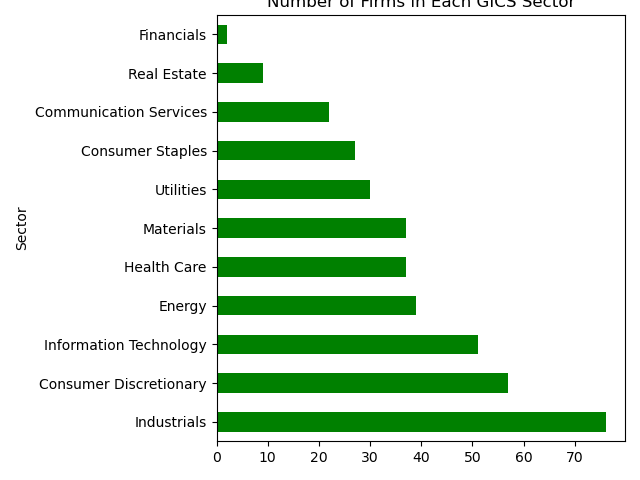
\includegraphics[width=\linewidth,keepaspectratio=true]{../Output/all_data_fixed_quarter_dates_firms_by_sector.png}
	\end{figure}

    sectoral imbalance

    outliers and errors

    correlations and patterns

    identification of good machine learning methods

    \section*{Modelling}

    began with logistic regression

    fitting and output

    assumptions
    
    interpretation

    \section*{Next Steps}

    more classifiers

    Graph Neural Network incorporating the relationships between companies, trained end-to-end with both tabular financial data and NLP features
    
    Fine tune the pre-trained LLMs for NLP feature construction
    
    Ensembling and Auto-ML
    
    \clearpage
    \newpage

    \bibliographystyle{chicago}
    \bibliography{Stat-222-Capstone}

    \clearpage
    \newpage

    \appendix

    \section*{Appendix}

\end{document}
